\chapter{Diseño del Sistema}

En este capítulo se presenta el diseño del sistema, que incluye el modelo de
dominio abordado, así como la arquitectura y el modelo de datos de la solución.

\section{Modelo de dominio}

La figura \ref{fig:modelo-dominio} muestra el modelo de dominio abordado, el cual ha
sido especificado utilizando UML. Allí se puede ver que la postulación es el
componente central del modelo. Ésta mantiene su estado, el postulante al cual
está asociada, la documentación adjunta, y todas las evaluaciones asociadas a
ella con su correspondiente evaluador. Uno de estos evaluadores es el
Coordinador del Programa, el cual emite una resolución acerca de la aceptación o
rechazo de la postulación al MTI.

\begin{figure}[!ht]
    \begin{center}
        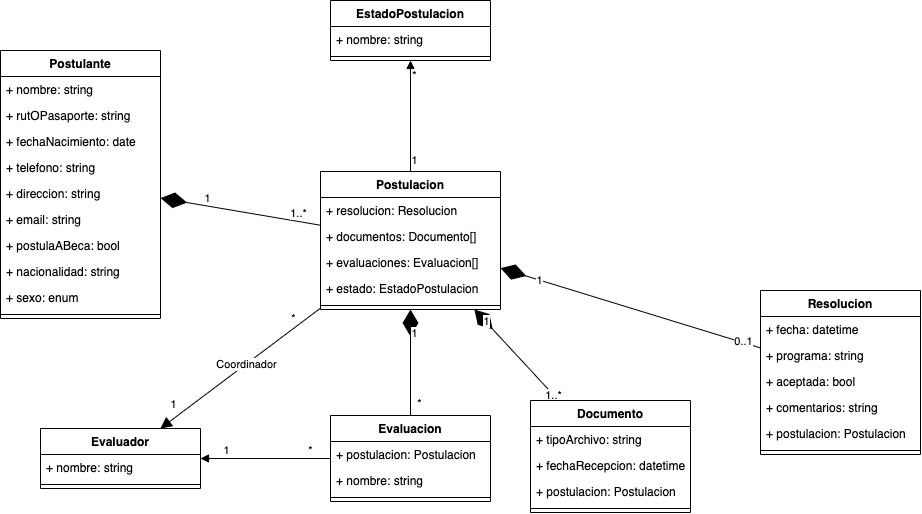
\includegraphics[scale=0.4]{imagenes/03-modelo-dominio.png}
    \end{center}
    \caption{Modelo de dominio del sistema}
    \label{fig:modelo-dominio}
\end{figure}

\section{Arquitectura del Sistema}

La Figura \ref{fig:arquitectura} muestra el modelo de contexto de la aplicación,
el cual representa el nivel de abstracción más alto en la representación de
arquitecturas según el modelo C4 [9]. Como se puede ver, los usuarios
interactúan con el sistema de evaluación de postulaciones al MTI, el cual extrae
los datos desde la aplicación web de UCampus. Esta arquitectura permite
independizar la forma de extraer datos, ya sea que esto se haga a través de una
API o a través de scrapers. El proceso de extracción de datos está encapsulado
un único módulo del sistema, lo cual permite reemplazarlo en caso de que a
futuro aparezcan mejores opciones para realizar la alimentación de datos.

\begin{figure}[!ht]
    \begin{center}
        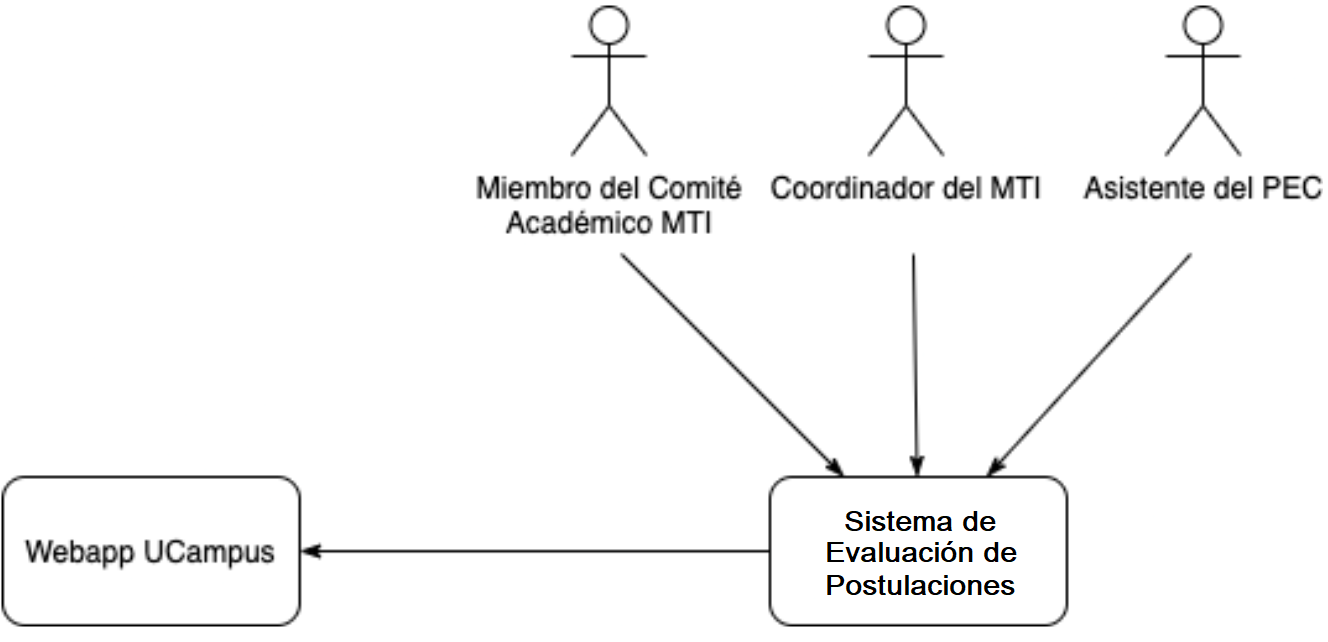
\includegraphics[scale=0.2]{imagenes/03-arquitectura.png}
    \end{center}
    \caption{Arquitectura general de la aplicación (Modelo de Contexto)}
    \label{fig:arquitectura}
\end{figure}

La Figura \ref{fig:descomposicion-sistema} muestra cómo está estructurado el
sistema en términos de sus macro-componentes y el repositorio de datos.
Particularmente, los usuarios del sistema interactúan con una aplicación
front-end, la cual contiene todas las interfaces de usuario del sistema. Ésta no
contiene la lógica de negocio, pues su rol es presentar la interfaz de usuario,
pedir datos al back-end, y mostrarlos al usuario.

Por otra parte, el back-end del sistema es el encargado de mantener la lógica de
la aplicación. En él se describen todos los procesos de negocio, y es el
encargado de la comunicación entre la interfaz de usuario y la base de datos. El
back-end además se comunica con la aplicación web de UCampus y extrae los datos
desde la página Web de postulaciones. Este componente es uno de los puntos más
críticos, pues es el que mantiene toda la lógica del sistema, y por lo tanto, es
el que ayuda a optimizar el proceso de postulaciones.

% El display de estas figuras es un desastre... mejorar

\begin{figure}[!ht]
    \begin{center}
        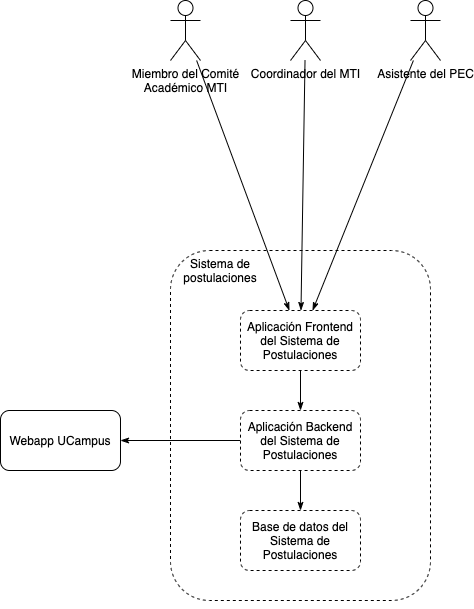
\includegraphics[scale=0.5]{imagenes/03-descomposicion-sistema.png}
    \end{center}
    \caption{Descomposición en componentes del Sistema de Evaluación de Postulaciones}
    \label{fig:descomposicion-sistema}
\end{figure}

Finalmente, la Figura \ref{fig:descomposicion-backend} muestra la descomposición
del back-end en sus principales componentes. Éste se divide en 4 componentes,
los cuales se describen a continuación.

\begin{figure}[!ht]
    \begin{center}
        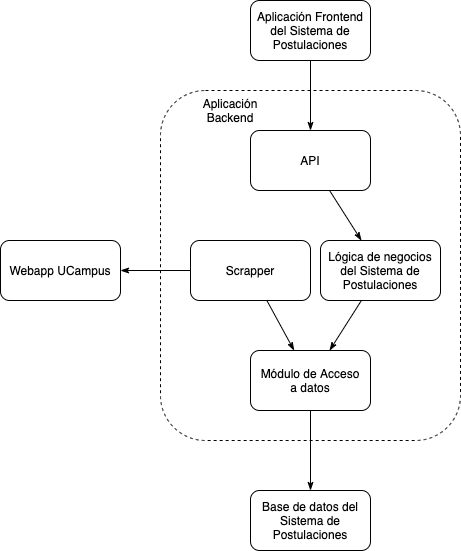
\includegraphics[scale=0.5]{imagenes/03-descomposicion-backend.png}
    \end{center}
    \caption{Descomposición en componentes del back-end del sistema (sólo se muestran los componentes relevantes).}
    \label{fig:descomposicion-backend}
\end{figure}

La \textbf{API} es un módulo HTTP encargado de disponibilizar los datos de la
aplicación para que puedan ser consumidos por la aplicación front-end. Este
módulo no contiene ninguna lógica; sólo sirve como medio de transporte de datos
desde y hacia la lógica de la aplicación. Por supuesto, este módulo también
recibe datos desde el front-end, y en dicho caso, es el encargado de transportar
esos datos hacia la capa de lógica de la aplicación.

Luego, el módulo de \textbf{lógica de negocios} es el encargado de implementar
el proceso y las interacciones de sus actores. En este módulo se puede encontrar
la lógica que procesa las postulaciones nuevas, crea las evaluaciones y recibe
los inputs de los actores del sistema.

El módulo de \textbf{acceso a datos} es el encargado de comunicarse con la base
de datos y persistir los datos que le llegan desde la lógica de negocio o desde
el scraper. Por último, el \textbf{scraper} es el módulo encargado de consumir
datos desde la página Web de UCampus, y enviarlos para que se almacenen en la
base de datos. Para ello, los datos que procesa el scraper son entregados como
input a la capa de acceso a datos. Vale la pena mencionar que los diagramas
antes presentados seguirán siendo válidos en el caso de que UCampus entregue los
datos de postulaciones vía una API para ser consumida por el sistema
desarrollado en esta memoria. La única cosa que cambiaría sería el uso de la
API, como reemplazo al actual uso del scraper.

\section{Modelo de Datos}

La figura \ref{fig:modelo-datos} muestra el modelo de datos del sistema, el cual
adhiere al modelo de dominio mostrado en la figura \ref{fig:modelo-dominio}.

\begin{figure}[!ht]
    \begin{center}
        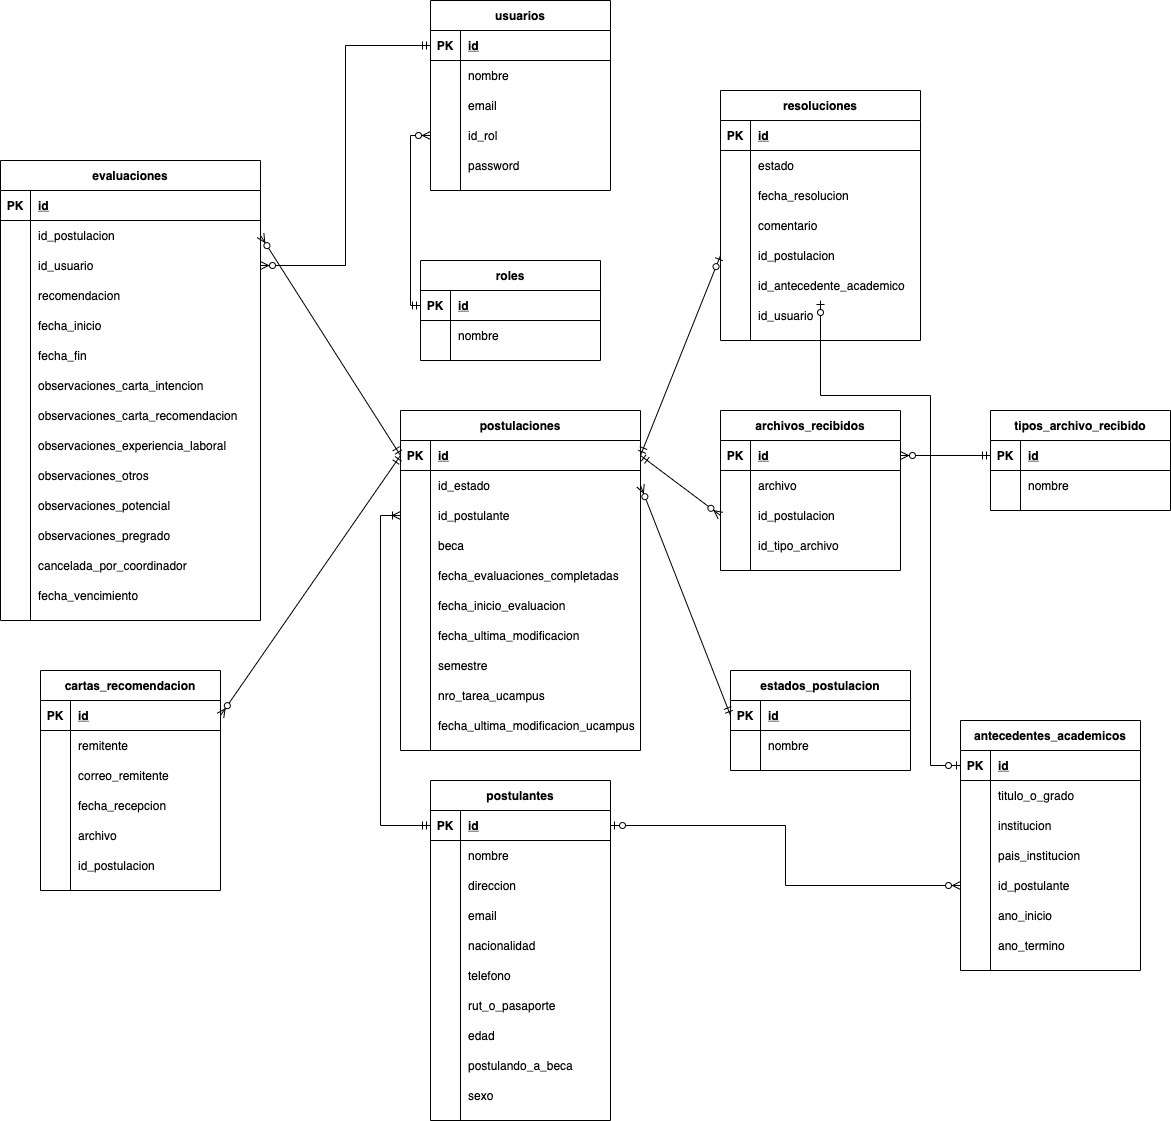
\includegraphics[scale=0.4]{imagenes/03-modelo-datos.png}
    \end{center}
    \caption{Modelo de datos del sistema}
    \label{fig:modelo-datos}
\end{figure}

En cada entidad de datos se puede ver los atributos de las mismas, cuyos nombres
son casi auto-explicativos. Tal como se ha mencionado antes, las postulaciones
son el centro neurálgico del sistema. Estas pertenecen a un postulante y tienen
documentación asociada (\texttt{cartas\_recomendacion} y
\texttt{archivos\_recibidos}, en Fig. \ref{fig:modelo-datos}). Además tienen
evaluaciones, un estado, y eventualmente resoluciones acerca de ellas, tal como
se indica en la figura. 

En el próximo capítulo se describe la implementación de este sistema.
